Atoms consist of a dense nucleus, composed of protons and neutrons, surrounded by electrons that do not follow classical trajectories. Instead of moving in well-defined orbits like planets around a star, electrons in atoms are described by orbitals: spatial distributions derived from the quantum mechanical wavefunction that give the probability of finding the electron in a given region.

These orbitals emerge as solutions to the Schrödinger equation applied to the Coulomb potential created by the positively charged nucleus. Each solution is characterized by a discrete set of parameters — the quantum numbers — which encode the electron's energy, spatial structure, and angular properties. There are four such quantum numbers:

\begin{itemize}[leftmargin=*]
  \item The \textbf{principal quantum number} $n = 1, 2, 3, \ldots$ determines the energy level and average radial extent of the orbital. Higher $n$ corresponds to greater distance from the nucleus and higher energy.
  \item The \textbf{angular momentum quantum number} $\ell = 0, 1, \ldots, n-1$ determines the orbital's shape. Values of $\ell$ are labeled spectroscopically as $s$ $(\ell=0)$, $p$ $(\ell=1)$, $d$ $(\ell=2)$, $f$ $(\ell=3)$, and continue alphabetically. For example, $s$ orbitals are spherically symmetric, while $p$ orbitals have a nodal plane and a dumbbell-like structure.
  \item The \textbf{magnetic quantum number} $m = -\ell, \ldots, +\ell$ defines the orientation of the orbital in space relative to a chosen axis (typically the $z$-axis).
  \item The \textbf{spin quantum number} $s = \pm \tfrac{1}{2}$ captures the intrinsic angular momentum of the electron, a quantum property with no classical analogue.
\end{itemize}

No two electrons in a single atom may occupy the same quantum state. This constraint — known as the Pauli exclusion principle — means that each combination $(n, \ell, m, s)$ can be occupied by at most one electron. For example, the $1s$ orbital can host two electrons: one with spin up and one with spin down.

\medskip

As electrons are added to an atom, they fill available orbitals according to energy minimization principles. This leads to the well-known electron filling sequence:
\[
1s,\ 2s,\ 2p,\ 3s,\ 3p,\ 4s,\ 3d,\ 4p,\ 5s,\ \ldots
\]
This order does not follow a strict progression in $n$, due to interactions such as shielding and penetration. Inner electrons partially screen the nucleus, reducing the effective nuclear charge experienced by outer electrons. Orbitals with the same $n$ but different $\ell$ values can therefore have different energies.

\medskip

To organize this structure, the following table summarizes the roles of each quantum number:

\begin{center}
\renewcommand{\arraystretch}{1.3}
\begin{tabular}{|c|c|c|c|c|}
\hline
\textbf{Name} & \textbf{Symbol} & \textbf{Allowed Values} & \textbf{Controls} & \textbf{Examples} \\
\hline
Principal & $n$ & $1, 2, 3, \ldots$ & Orbital energy and size & $1s,\ 2p,\ 4d$ \\
Angular Momentum & $\ell$ & $0 \leq \ell < n$ & Shape & $s,\ p,\ d,\ f$ \\
Magnetic & $m$ & $-\ell \leq m \leq +\ell$ & Spatial orientation & $p_x,\ p_y,\ p_z$ \\
Spin & $s$ & $\pm \tfrac{1}{2}$ & Electron spin & $\uparrow,\ \downarrow$ \\
\hline
\end{tabular}
\end{center}

\medskip

In hydrogen-like atoms (single electron, full nuclear charge), all orbitals with the same $n$ are degenerate — they have the same energy regardless of $\ell$. This symmetry is broken in multi-electron atoms, where electron–electron repulsion and the shape of orbitals result in energy level splitting.

Orbital shapes are determined by both radial and angular structure. The radial part depends on $n$ and $\ell$, while the angular part (controlled by $m$ and $\ell$) determines nodal planes and symmetry axes. For instance, a $3d$ orbital has two angular nodes and occupies a region shaped like a cloverleaf.

\medskip

The periodic table reflects these principles. Each row corresponds roughly to a value of $n$, and the structure of each column — especially among main-group elements — reflects the number and configuration of valence electrons, those in the outermost shell. Elements with similar valence configurations (e.g., noble gases, alkali metals) exhibit analogous chemical properties.

\medskip

The color and optical appearance of a material are determined by how it interacts with light. Light is an electromagnetic wave, characterized by its wavelength \( \lambda \). When light strikes a material, some wavelengths may be absorbed, while others are reflected or transmitted. The observed color corresponds to the reflected portion of the spectrum. For instance, a substance that absorbs blue light and reflects red and green will appear yellow. The mechanism behind absorption is electronic: photons transfer their energy to electrons, promoting them from lower to higher energy states.

This promotion can only occur if the photon's energy matches the gap between two allowed electronic states. Since atomic orbitals are quantized, so are the possible energy differences. The energy of a photon is given by the Planck-Einstein relation:
\[
E = \frac{hc}{\lambda},
\]
where \( h \) is Planck’s constant and \( c \) is the speed of light. Shorter wavelengths (such as blue or violet) correspond to higher photon energies, while longer wavelengths (such as red or infrared) correspond to lower energies. If the energy gap between two orbitals aligns with the energy of a visible photon, that wavelength may be absorbed. The pattern of these absorptions defines the material’s optical spectrum and determines its visual appearance.

Now let's talk relativity. Special relativity describes the behavior of physical systems at speeds approaching the speed of light \( c \). Its core insight is that measurements of time, length, and mass depend on the observer’s inertial frame. For a particle with rest mass \( m_0 \), the effective mass increases with velocity according to the expression:
\[
m_\text{eff} = \frac{m_0}{\sqrt{1 - v^2/c^2}}.
\]
This formula implies that as \( v \to c \), the ratio \( v^2/c^2 \) approaches 1, causing the denominator \( \sqrt{1 - v^2/c^2} \) to shrink toward zero. Thus, the effective mass \( m_\text{eff} \) increases without bound. Physically, this means that accelerating a particle closer to the speed of light requires more and more energy, and reaching \( v = c \) would require infinite energy. As a result, no object with nonzero rest mass can be accelerated to the speed of light.

In practice, even modest fractions of \( c \) can result in measurable mass increase and energy shifts. For example, at \( v/c = 0.6 \), the denominator becomes \( \sqrt{1 - 0.36} = 0.8 \), so the effective mass is increased by a factor of \( 1/0.8 = 1.25 \). These corrections are small for everyday objects but become significant for subatomic particles, especially in high-energy regimes such as atomic orbitals in heavy atoms.

When considering electrons in atoms, however, the notion of velocity must be interpreted within quantum mechanics. Electrons in bound states do not follow classical trajectories. Their behavior is described by wavefunctions, and dynamical quantities — such as momentum or velocity — are represented by operators acting on those wavefunctions. In non-relativistic quantum mechanics, the velocity operator is given by:
\[
\hat{v} = \frac{\hat{p}}{m_0}, \quad \text{where} \quad \hat{p} = -i\hbar \nabla.
\]
The expectation value \( \langle \hat{v} \rangle \) offers a statistical measure of the electron’s effective motion within the orbital. While it does not describe a definite speed or path, it provides a meaningful average scale for kinetic behavior.

For hydrogen-like atoms — idealized atoms with a single electron and full nuclear charge — the expectation value of electron velocity in atomic units scales approximately as:
\[
\langle v \rangle \sim Z\alpha c,
\]
where \( Z \) is the atomic number — the number of protons in the nucleus — and \( \alpha \approx \tfrac{1}{137} \) is the fine-structure constant. This relation captures the intuition that electrons are drawn more tightly and accelerated more strongly in atoms with higher nuclear charge. As \( Z \) increases, the electron’s velocity increases proportionally, and the resulting relativistic mass correction becomes non-negligible.

These relativistic effects modify the quantum mechanical equations that describe bound states. In particular, the Schrödinger equation must be replaced or augmented by relativistic formulations such as the Dirac equation. These corrections shift the energies and shapes of orbitals, even in the absence of external fields. The resulting deviations from non-relativistic predictions grow systematically with atomic number and are especially significant for the inner (core) electrons in heavy elements.

Relativistic quantum chemistry incorporates these effects into the modeling of atoms and molecules. In this framework, changes in orbital shape and energy are direct consequences of relativistic dynamics applied to quantum-bound electrons. While negligible in light atoms, these corrections become essential to accurately describing the physical properties of high-$Z$ elements.

In most metals, optical behavior is dominated by conduction electrons. These electrons are not localized to individual atoms but move freely through the crystal, occupying partially filled energy bands. Because these conduction bands are broad and continuous, they allow electrons to respond uniformly to incoming electromagnetic waves. As a result, nearly all visible wavelengths are reflected equally, and the metal appears silvery or white. This is why typical metals, such as aluminum, iron, or silver, lack color: their optical response is effectively achromatic.

However, when deeper (non-conduction) bands lie close to the Fermi level (the highest occupied energy level at absolute zero) interband transitions become possible. In this case, photons can excite electrons from filled lower bands (such as d-bands) into the conduction band, but only if their energy matches the band gap. If this gap lies within the visible range, the metal absorbs specific wavelengths and reflects the rest, producing color.

In gold and other heavy elements, relativistic effects shift the energies of these bands. s-orbitals contract due to high nuclear charge, while d-orbitals remain more diffuse. This reduces the energy difference between them and brings the d-to-s gap into the visible spectrum.

In silver ($Z = 47$), relativistic effects are minor. The 4d band lies well below the Fermi level, and interband transitions require photon energies above the visible range. As a result, silver reflects nearly all visible light uniformly and appears bright white.

In gold ($Z = 79$), relativistic contraction of the 6s orbital lowers the conduction band, while expansion and destabilization of the 5d orbitals raises the valence band. The gap between them narrows to be significantly smaller than the non-relativistic prediction of around 3.7 eV: $_{\text{5d} \to \text{6s}} \approx 2.4\ \text{eV}.$

which corresponds to an absorption wavelength of:

$$
\lambda \approx \frac{1240\ \text{eV}\cdot\text{nm}}{2.4\ \text{eV}} \approx 520\ \text{nm}.
$$

This lies in the blue region of the spectrum. Because the 5d and 6s bands are broad, many interband transitions occur across a range of energies. The absorption is therefore not narrow, but spread slightly, selectively removing blue light from the reflected spectrum. The result is gold’s distinctive yellow color, enriched in red and green wavelengths.

\pgfplotsset{
  colormap={visiblespectrum}{
    color(0cm)=(red);
    color(1cm)=(orange);
    color(2cm)=(yellow);
    color(3cm)=(green);
    color(4cm)=(cyan);
    color(5cm)=(blue);
    color(6cm)=(violet);
  }
}



\begin{figure}[h]
\centering
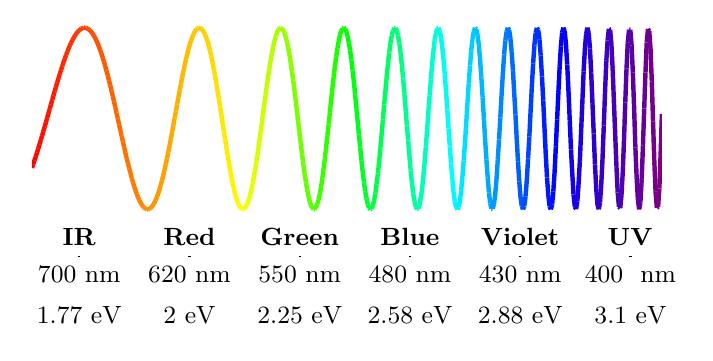
\begin{tikzpicture}
  % Rainbow plot using pgfplots with correct scale
  \begin{axis}[
    hide axis,
    scale=1,
    domain=2.6:3.6,
    samples=500,
    xmin=2.6, xmax=3.6,
    ymin=-0.26, ymax=0.26,
    scale only axis,
    width=8cm,
    height=3cm,
    every axis/.append style={scale=1}
  ]
    \addplot[
      mesh,
      ultra thick,
      point meta=x,
      colormap name=visiblespectrum
    ] {sin(deg(x^x))/5};
  \end{axis}
  
  % Horizontal bounds - adjusted with coordinates
  %\draw[dashed] (0.6,0.25) -- (8.6,0.25);
  %\draw[dashed] (0.6,-0.25) -- (8.6,-0.25);
  
  % Top labels: Color names
  \foreach \x/\pos/\label in {
    2.6/0.6/IR, 2.8/2.0/Red, 3.0/3.4/Green, 3.2/4.8/Blue, 3.4/6.2/Violet, 3.6/7.6/UV
  } {
    
    \node at (\pos,0) {\small \textbf{\label}};
    
  }
  
  % Bottom labels: nm values and calculated eV values
  \foreach \pos/\nm in {
    0.6/700, 2.0/620, 3.4/550, 4.8/480, 6.2/430, 7.6/400
  } {
    \draw[thick] (\pos,-0.26) -- (\pos,-0.25);
    \node[below] at (\pos,-0.26) {\small \nm~nm};
    
    % Calculate eV from nm: eV = 1240/nm
    \pgfmathparse{1240/\nm}
    \edef\ev{\pgfmathresult}
    \node[below=0.5cm] at (\pos,-0.26) {\small \pgfmathprintnumber[fixed, precision=2]{\ev}~eV};
    
  }
\end{tikzpicture}
\end{figure}

Platinum ($Z = 78$) also experiences strong relativistic shifts, but its partially filled 5d$^9$ configuration and broader interband spacing push absorption into the ultraviolet. Thus, platinum reflects visible light uniformly and appears silvery-white.

Copper ($Z = 29$), though far lighter, has a naturally narrow d–s gap of about 2.1 eV even without relativistic effects. This gap also falls within the visible range and leads to selective absorption of blue-green wavelengths, producing its reddish hue.

Mercury ($Z = 80$) reveals a different consequence of relativistic orbital shifts. The 6s orbital contracts so strongly that its electrons become tightly bound and chemically inert. This severely reduces orbital overlap and weakens metallic bonding. The result is a low cohesive energy and an anomalously low melting point. Mercury remains liquid at room temperature — a phase behavior that non-relativistic models cannot reproduce.

\clearpage

These orbital transitions can be visualized as shifts in energy bands across different elements:

\usetikzlibrary{arrows.meta, positioning, backgrounds, calc}

\definecolor{copperfill}{RGB}{205, 127, 50}
\definecolor{silverfill}{RGB}{230, 230, 230}
\definecolor{goldfill}{RGB}{255, 215, 0}
\definecolor{platinumfill}{RGB}{180, 180, 200}
\definecolor{paneloutline}{RGB}{51, 51, 51}

\begin{figure}[H]
\centering
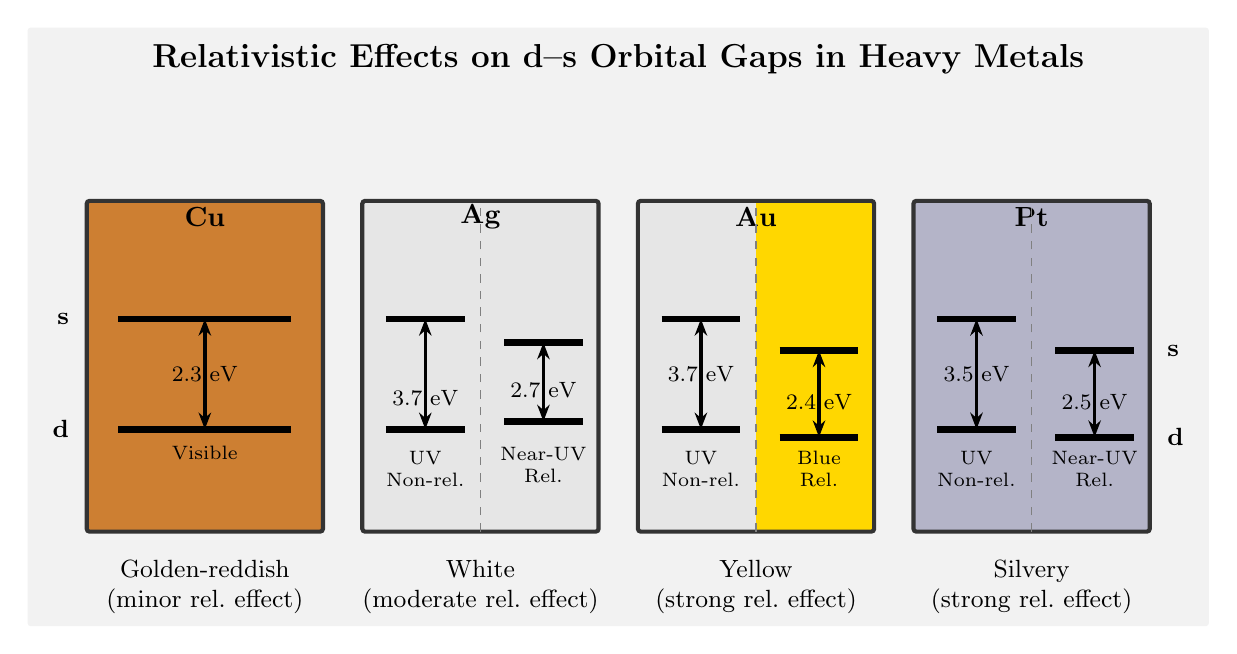
\begin{tikzpicture}[
  panel/.style       ={rounded corners=1pt, draw=paneloutline, line width=1.5pt},
  copper/.style      ={panel, fill=copperfill},
  silver/.style      ={panel, fill=silverfill},
  gold/.style        ={panel},
  platinum/.style    ={panel, fill=platinumfill},
  title/.style       ={font=\bfseries\large},
  metal-name/.style  ={font=\bfseries\normalsize},
  appearance/.style  ={font=\small, align=center},
  energy-band/.style ={line width=2.5pt},
  reverse-transition/.style={{Stealth[length=6pt]}-{Stealth[length=6pt]}, line width=1.2pt},
  energy-label/.style={font=\footnotesize},
  light-type/.style  ={font=\scriptsize, align=center},
  orbital-guide/.style={font=\bfseries\small},
  concept-detail/.style={font=\scriptsize, align=center},
  divider/.style     ={dashed, gray}
]

% Panel dimensions and positioning
\def\w{3}
\def\xCu{0.25}
\def\xAg{3.75}
\def\xAu{7.25}
\def\xPt{10.75}
\def\panelTop{5.4}

% Background
\fill[gray!10, rounded corners=1pt] (-0.5,0) rectangle (14.5,7.6);

% Title
\node[title] at (\xCu+6.75,7.2) {Relativistic Effects on d--s Orbital Gaps in Heavy Metals};

% Orbital guides
\node[orbital-guide, anchor=east] at (\xCu-0.1,3.9) {s};
\node[orbital-guide, anchor=east] at (\xCu-0.1,2.5) {d};
\node[orbital-guide, anchor=west] at (\xPt+\w+0.1,3.5) {s};
\node[orbital-guide, anchor=west] at (\xPt+\w+0.1,2.4) {d};

% ---------------------- Cu ----------------------
\draw[copper] (\xCu,1.2) rectangle ++(\w,4.2);
\node[metal-name] at (\xCu+1.5,5.2) {Cu};
\draw[energy-band] (\xCu+0.4,3.9) -- ++(2.2,0);
\draw[energy-band] (\xCu+0.4,2.5) -- ++(2.2,0);
\draw[reverse-transition] (\xCu+1.5,3.9) -- ++(0,-1.4);
\node[energy-label] at (\xCu+1.5,3.2) {2.3 eV};
\node[light-type] at (\xCu+1.5,2.2) {Visible};
\node[appearance] at (\xCu+1.5,0.5) {Golden-reddish\\(minor rel.\ effect)};

% ---------------------- Ag ----------------------
\draw[silver] (\xAg,1.2) rectangle ++(\w,4.2);
\node[metal-name] at (\xAg+1.5,5.2) {Ag};
\draw[divider] (\xAg+1.5,1.2) -- (\xAg+1.5,\panelTop);

% Non-rel
\draw[energy-band] (\xAg+0.3,3.9) -- ++(1.0,0);
\draw[energy-band] (\xAg+0.3,2.5) -- ++(1.0,0);
\draw[reverse-transition] (\xAg+0.8,3.9) -- ++(0,-1.4);
\node[energy-label] at (\xAg+0.8,2.9) {3.7 eV};
\node[light-type] at (\xAg+0.8,2.0) {UV\\Non-rel.};

% Rel
\draw[energy-band] (\xAg+1.8,3.6) -- ++(1.0,0);
\draw[energy-band] (\xAg+1.8,2.6) -- ++(1.0,0);
\draw[reverse-transition] (\xAg+2.3,3.6) -- ++(0,-1.0);
\node[energy-label] at (\xAg+2.3,3.0) {2.7 eV};
\node[light-type] at (\xAg+2.3,2.05) {Near-UV\\Rel.};
\node[appearance] at (\xAg+1.5,0.5) {White\\(moderate rel.\ effect)};

% ---------------------- Au ----------------------
\path[fill=silverfill] (\xAu,1.2) rectangle ++(1.5,4.2);
\path[fill=goldfill]   (\xAu+1.5,1.2) rectangle ++(1.5,4.2);
\draw[gold] (\xAu,1.2) rectangle ++(\w,4.2);
\node[metal-name] at (\xAu+1.5,5.2) {Au};
\draw[divider] (\xAu+1.5,1.2) -- (\xAu+1.5,\panelTop);

% Non-rel
\draw[energy-band] (\xAu+0.3,3.9) -- ++(1.0,0);
\draw[energy-band] (\xAu+0.3,2.5) -- ++(1.0,0);
\draw[reverse-transition] (\xAu+0.8,3.9) -- ++(0,-1.4);
\node[energy-label] at (\xAu+0.8,3.2) {3.7 eV};
\node[light-type] at (\xAu+0.8,2) {UV\\Non-rel.};

% Rel
\draw[energy-band] (\xAu+1.8,3.5) -- ++(1.0,0);
\draw[energy-band] (\xAu+1.8,2.4) -- ++(1.0,0);
\draw[reverse-transition] (\xAu+2.3,3.5) -- ++(0,-1.1);
\node[energy-label] at (\xAu+2.3,2.85) {2.4 eV};
\node[light-type] at (\xAu+2.3,2) {Blue\\Rel.};
\node[appearance] at (\xAu+1.5,0.5) {Yellow\\(strong rel.\ effect)};

% ---------------------- Pt ----------------------
\draw[platinum] (\xPt,1.2) rectangle ++(\w,4.2);
\node[metal-name] at (\xPt+1.5,5.2) {Pt};
\draw[divider] (\xPt+1.5,1.2) -- (\xPt+1.5,\panelTop);

% Non-rel
\draw[energy-band] (\xPt+0.3,3.9) -- ++(1.0,0);
\draw[energy-band] (\xPt+0.3,2.5) -- ++(1.0,0);
\draw[reverse-transition] (\xPt+0.8,3.9) -- ++(0,-1.4);
\node[energy-label] at (\xPt+0.8,3.2) {3.5 eV};
\node[light-type] at (\xPt+0.8,2) {UV\\Non-rel.};

% Rel
\draw[energy-band] (\xPt+1.8,3.5) -- ++(1.0,0);
\draw[energy-band] (\xPt+1.8,2.4) -- ++(1.0,0);
\draw[reverse-transition] (\xPt+2.3,3.5) -- ++(0,-1.1);
\node[energy-label] at (\xPt+2.3,2.85) {2.5 eV};
\node[light-type] at (\xPt+2.3,2) {Near-UV\\Rel.};
\node[appearance] at (\xPt+1.5,0.5) {Silvery\\(strong rel.\ effect)};

% Caption

\end{tikzpicture}
\label{fig:relativistic_energy_levels_final}
\end{figure}


\begin{commentary}[Commentary: Low-Limit Theories]
Usually in physical sciences, there are simplifications to the precise theories that are applicable when one "zooms out." For example, at low velocities, there is no need for the relativistic formulation of addition of velocities, and one uses the Galilean formulation. In low mass scenarios (and interactions of objects with Earth are usually considered to have low enough mass), Newtonian gravity rules are sufficient.

These approximations or \textbf{"low-limit theories"} have well-defined domains of validity. Classical mechanics is valid when $v \ll c$; Newtonian gravity applies when gravitational fields are weak; geometrical optics works when wavelengths are much smaller than object dimensions. The transition between these regimes is often characterized by dimensionless parameters — the ratio of velocity to light speed ($v/c$), the gravitational potential ($GM/rc^2$), or the ratio of wavelength to object size ($\lambda/L$). When these parameters approach unity, the simplified theories break down.

The scale at which these "low-limit theories" work changes with the theory, but in mechanics one typically uses classical physics, and in chemistry, simplistic models of the atom (electrons "orbiting" a positive nucleus) are adequate for most organic and inorganic chemistry applications.

Still, sometimes lower-level theories and not averaging theories are needed. \textbf{This is why it is interesting that for something as common as the color of gold, the theory that explains it relies on relativistic corrections}. The relativistic effects on electron orbitals in gold atoms directly influence its optical properties, causing it to absorb blue light and appear yellow, whereas a non-relativistic prediction would result in gold having a silvery appearance like neighboring elements in the periodic table.

It is rare to need special relativity to explain macroscopic phenomena we encounter daily. Most everyday objects move at speeds vastly slower than light, and relativistic effects are negligible. This is what makes the gold example particularly noteworthy — it represents one of the few cases where a macroscopic property (color) can only be correctly predicted by including special relativistic effects. Without these corrections, our theoretical models would make an incorrect prediction about a common observation.
\end{commentary}

\thispagestyle{empty}
\begin{figure}[p]
\centering
\fbox{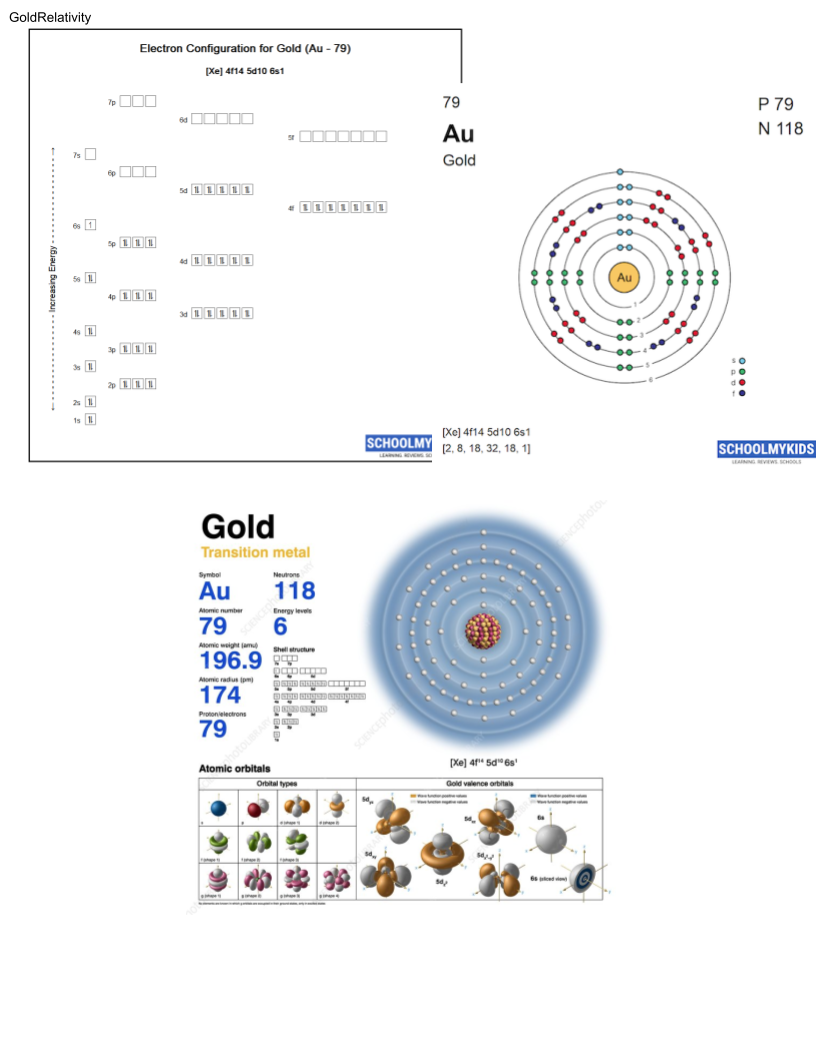
\includegraphics[width=\textwidth,height=\textheight,keepaspectratio]{03_GoldRelativity/gold_illus.png}}
\end{figure}

